\chapter{Results}\label{sec:results}

\section{Filtering out noise}\label{sec:noise}
After the tracking and stitching steps are completed, the algorithm results can
still be improved by filtering the results. A large improvement was
achieved by requiring a certain sea surface temperature at TC genesis.
\subsection*{Sea Surface Temperature Criterion}
As outlined in Sec.~\ref{sec:physics}, the TCs need warm ocean water as an
energy source, when they form. It has been shown that the large
majority has an SST over 25.5\degree C \cite{sst-paper}. Therefore it is
expected that no reasonable TCs are filtered out when requiring a genesis SST
of at least 24\degree C. However, as can be seen in Fig.~\ref{fig:sst-effect},
a large part of the unwanted tracks in the North of the domain are removed.
% TODO ?? use figures here and in general with reasonable and elaborated parameters only
\begin{figure}[ht]
	\begin{minipage}[t]{0.48\textwidth}
		\includegraphics[width = \textwidth]{img/all_tracks.png}
	\end{minipage}
	\hfill
	\begin{minipage}[t]{0.48\textwidth}
		\includegraphics[width = \textwidth]{img/all_tracks_sst.png}
	\end{minipage}
	\caption{Comparison of all tracks without and with the SST criterion on the left and right}
	\label{fig:sst-effect}
\end{figure}

\subsection*{Analysing geographically unreasonable tracks}
Even with the application of the SST-criterion, unreasonable TC tracks remain. For instance the tracks over Wyoming shown in Fig.~\ref{fig:rogue-tracks} should not be so frequent. To determine the parameters responsible for this, the 20 parameter combinations that account for the large majority of these, share the common feature that they all correspond to the same weak warm core criterion. They had a \textbf{temdif} of \unit[0.5]{\degree C} and a \textbf{temdis} of \unit[400]{km}. Therefore if only a very low temperature difference is required for an area that can be larger than smaller-sized TCs, low pressure systems that do not correspond to tropical cyclones are tracked. While this may not be surprising, it does emphasise the importance of a well-trimmed warm core criterion.
% TODO Change Category -1 to tropical depression and 0 to tropical storm
\begin{figure}[ht]
	\centering
	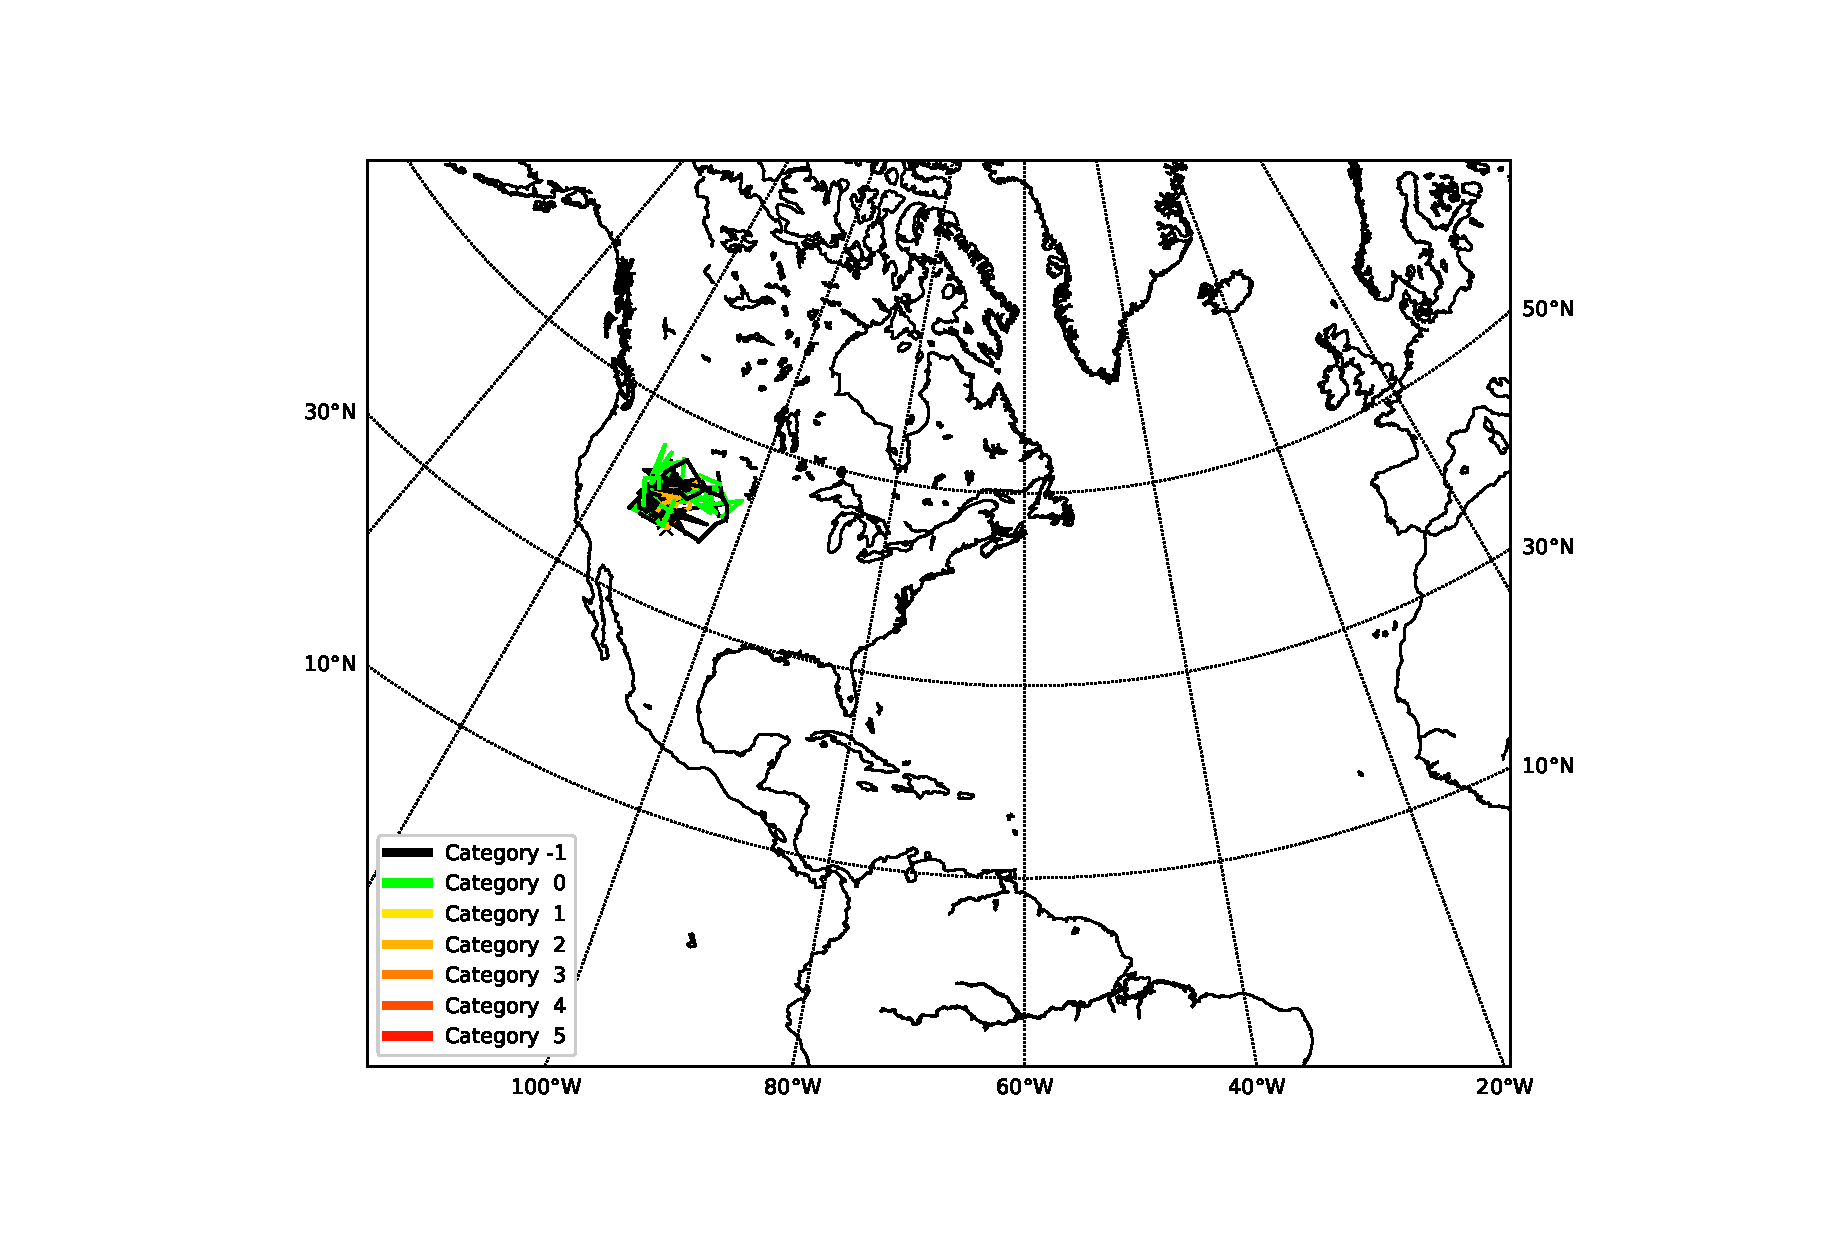
\includegraphics[width=0.7\textwidth]{img/rogue_tracks.eps}
	\caption{Set of unreasonable tracks over Wyoming and the surrounding states}
	\label{fig:rogue-tracks}
\end{figure}
\section{Validating Results}
In Sec.~\ref{sec:noise}, it was found that with a sufficiently strong warm core condition the tracks appear in reasonable areas. Before comparing the algorithm output for different parameter combinations, it still remains to be shown that the produced tracks actually follow TCs and not other low pressure systems. For this purpose, ten different storms were randomly chosen. For these storms the radial, tangential and vertical wind and the sea level pressure were visualised in the azimuthal mean. It was found that all storms qualitatively exhibit the physically expected structure that was described in Sec.~\ref{sec:physics}. The resulting plots for a representative storm can be seen in Fig.~\ref{fig:azimean}.

\begin{figure}[ht]
	\centering
	\begin{subfigure}{.5\linewidth}
		\centering
		\includegraphics[width=0.75\linewidth]{img/tight09279566radwind20130706T120000Z.eps}
	\end{subfigure}%
	\begin{subfigure}{.5\linewidth}
		\centering
		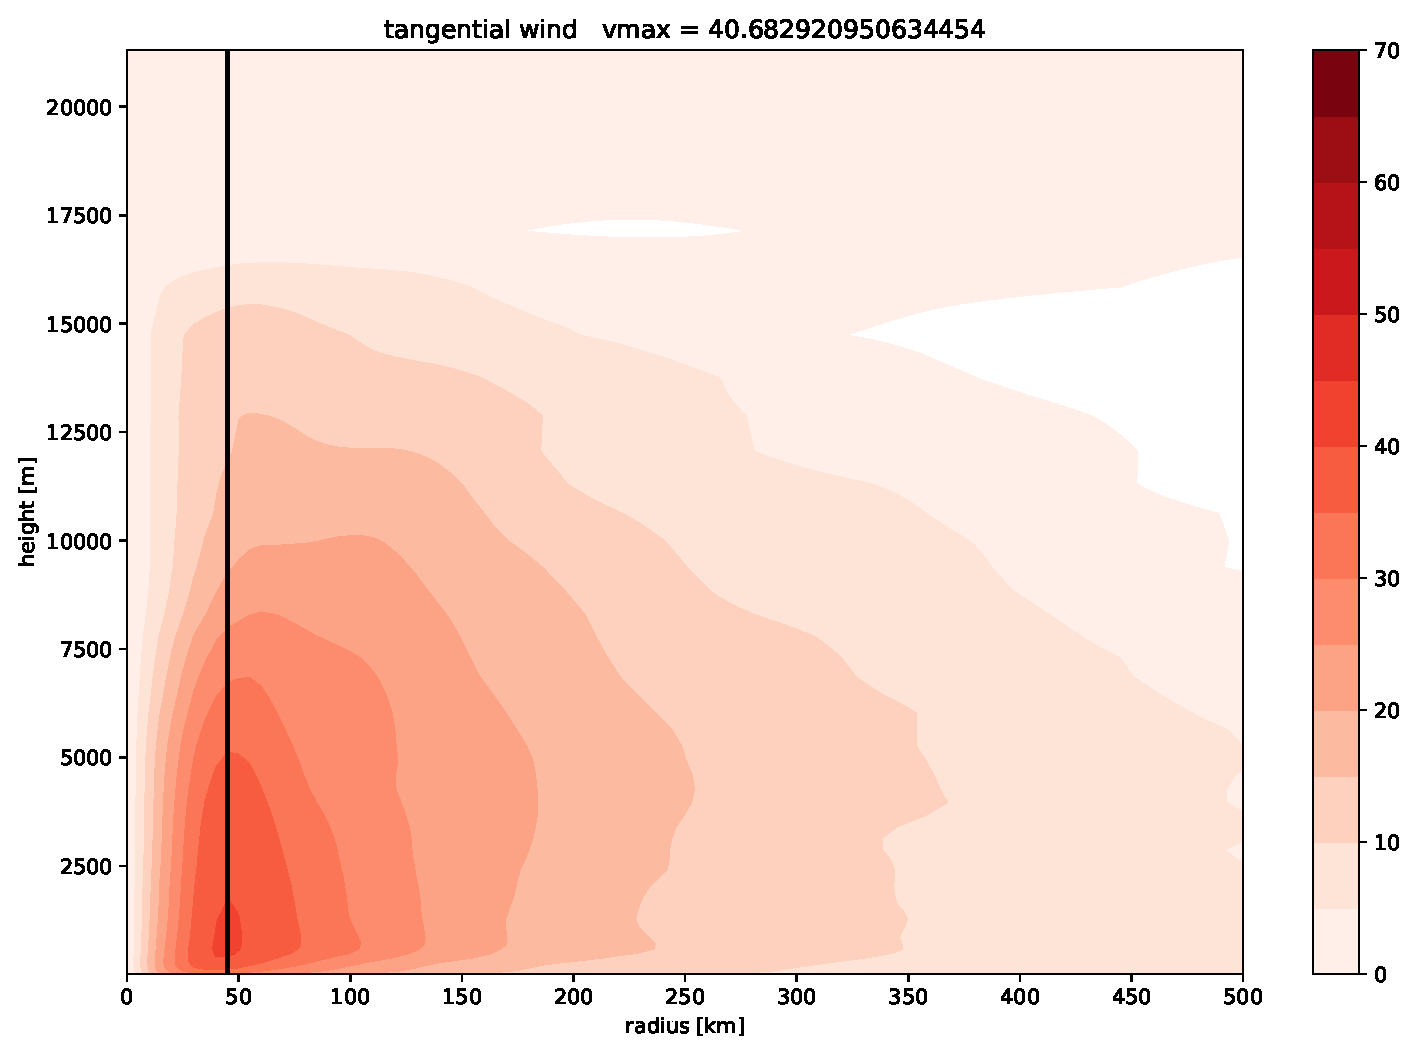
\includegraphics[width=0.75\linewidth]{img/tight09279566tanwind20130706T120000Z.eps}
	\end{subfigure}
	\begin{subfigure}{.5\linewidth}
		\centering
		\includegraphics[width=0.75\linewidth]{img/tight09279566verwind20130706T120000Z.eps}
	\end{subfigure}%
	\begin{subfigure}{.5\linewidth}
		\centering
		\includegraphics[width=0.75\linewidth]{img/tight09279566pres_msl20130706T120000Z.eps}
	\end{subfigure}
	\caption[short]{Azimuthal mean plots. From left to right and top to bottom: radial wind, tangential wind, vertical wind and sea level pressure. The vertical black line marks the radius of maximum wind.}
	\label{fig:azimean}
\end{figure}
% TODO ADD TEMPERATURE ANOMALY


\section{Variation of the Warm Core Criterion strength}
With the aim of understanding the impact of different warm core criteria strengths, the resulting cyclone distributions for a range of different \textbf{temdif} values were compared. As can be seen in Fig.~\ref{fig:temdif-analysis}, a weaker warm core criterion leads to a distribution with more lower-intensity storms. When comparing with the absolute counts, it can be seen that this is the result from weaker storms being tracked for lower \textbf{temdif}s. Logically, for TCs of category 2 and upwards, no difference in the counts is observed. Furthermore for \textbf{temdif}s larger than \unit[1]{K}, no tropical depressions which correspond to category -1 are tracked. It can therefore be concluded that the warm core criterion can be used very efficiently to filter out noise if only strong TCs are of interest.

\begin{figure}[ht]
	\begin{minipage}[t]{0.48\textwidth}
		\includegraphics[width = \textwidth]{img/max_cat_distr_temdifs.eps}
	\end{minipage}
	\hfill
	\begin{minipage}[t]{0.48\textwidth}
		\includegraphics[width = \textwidth]{img/max_cat_counts_temdifs.eps}
	\end{minipage}
	\caption{Maximum TC category histograms for different \textbf{temdif} parameters. Each histogram on the left has unit norm. The right plot shows the absolute counts of TCs. The X-axis describes the TC categories as defined in Tab~\ref{tab:simpson-scale}. Comparing the normalised distributions on the left with the absolute counts on the right shows the good agreement of the algorithm for different values of \textbf{temdif} on strong TCs and the heavier weight on lower category storms for the lower \textbf{temdif} values.}
	\label{fig:temdif-analysis}
\end{figure}
% TODO move description to text and write about lower tailed and higher tailed distribtuion or sth else pseudo statistical


\section{Comparison of the Warm Core Criterion and the Vorticity Threshold}\label{sec:warmcore-var}
In order to compare the importance of the warm core criterion with the vorticity threshold, only the TC tracks that were found using the parameter combinations from Tab.~\ref{tab:vor-tem-comparison} were analysed. These combinations were chosen because they correspond to different relative strengths of the two criteria.

\begin{table}[ht]
	\centering
	\begin{tabular}{|l|l|l|}
		\hline
		\textbf{parameter} & \textbf{unit} & \textbf{values}  \\ \hline
		slpdis             & m             & 100000           \\
		vormin             & 1/s           & 1e-6, 1e-5, 1e-4 \\
		temdif             & K             & 0.5, 1 ,1.5      \\
		temdis             & m             & 200000           \\ \hline
	\end{tabular}
	\caption{Parameter combinations used for the comparison}
	\label{tab:vor-tem-comparison}
\end{table}

It was expected that the vorticity threshold should influence the distribution of tracked TCs only if a weak warm core criterion is applied. This was hypothesised because most low pressure systems with strong warm cores should exhibit the necessary minimum vorticity while weak warm core systems might not have a strong enough rotating motion. However, as can be seen in Fig.~\ref{fig:temdif-vormin-comp}, even with a very weak warm core criterion does the vorticity threshold not influence the storm intensity distributions. A comparison for different values of \textbf{temdif} and an analysis of the impact of the vorticity criterion on the storm lifetime can be found in the Appendix.
\begin{figure}[ht]
	\centering
	\includegraphics[width=0.7\textwidth]{img/curr_category_vortem05.eps}
	\caption{Snapshot category distribution for a weak warm core criterion and several vorticity thresholds. The Y-axis shows the normalised counts.}
	\label{fig:temdif-vormin-comp}
\end{figure}
% TODO fix max and snapshot category contradiction


\section{TC Genesis regions}
A direct consequence of the observations from Sec.~\ref{sec:warmcore-var} is that with a weaker warm core criterion the TCs can be found already when they have not had much time to intensify. This is relevant because from best track data it is expected that most TCs form in the main development region (MDR) which lies roughly between 10 -- 20 \degree N and 20 -- 80 \degree W. However, when checking the genesis locations and density in Fig.~\ref{fig:genesis-temdif1}, it can be seen that the formation of TCs in ICON is not limited to the MDR. When using a weaker warm core criterion, the areas of highest TC density shift more towards the expected region. This can be interpreted as the successful detection of TCs in earlier development phases.
\begin{figure}[ht]
	\centering
	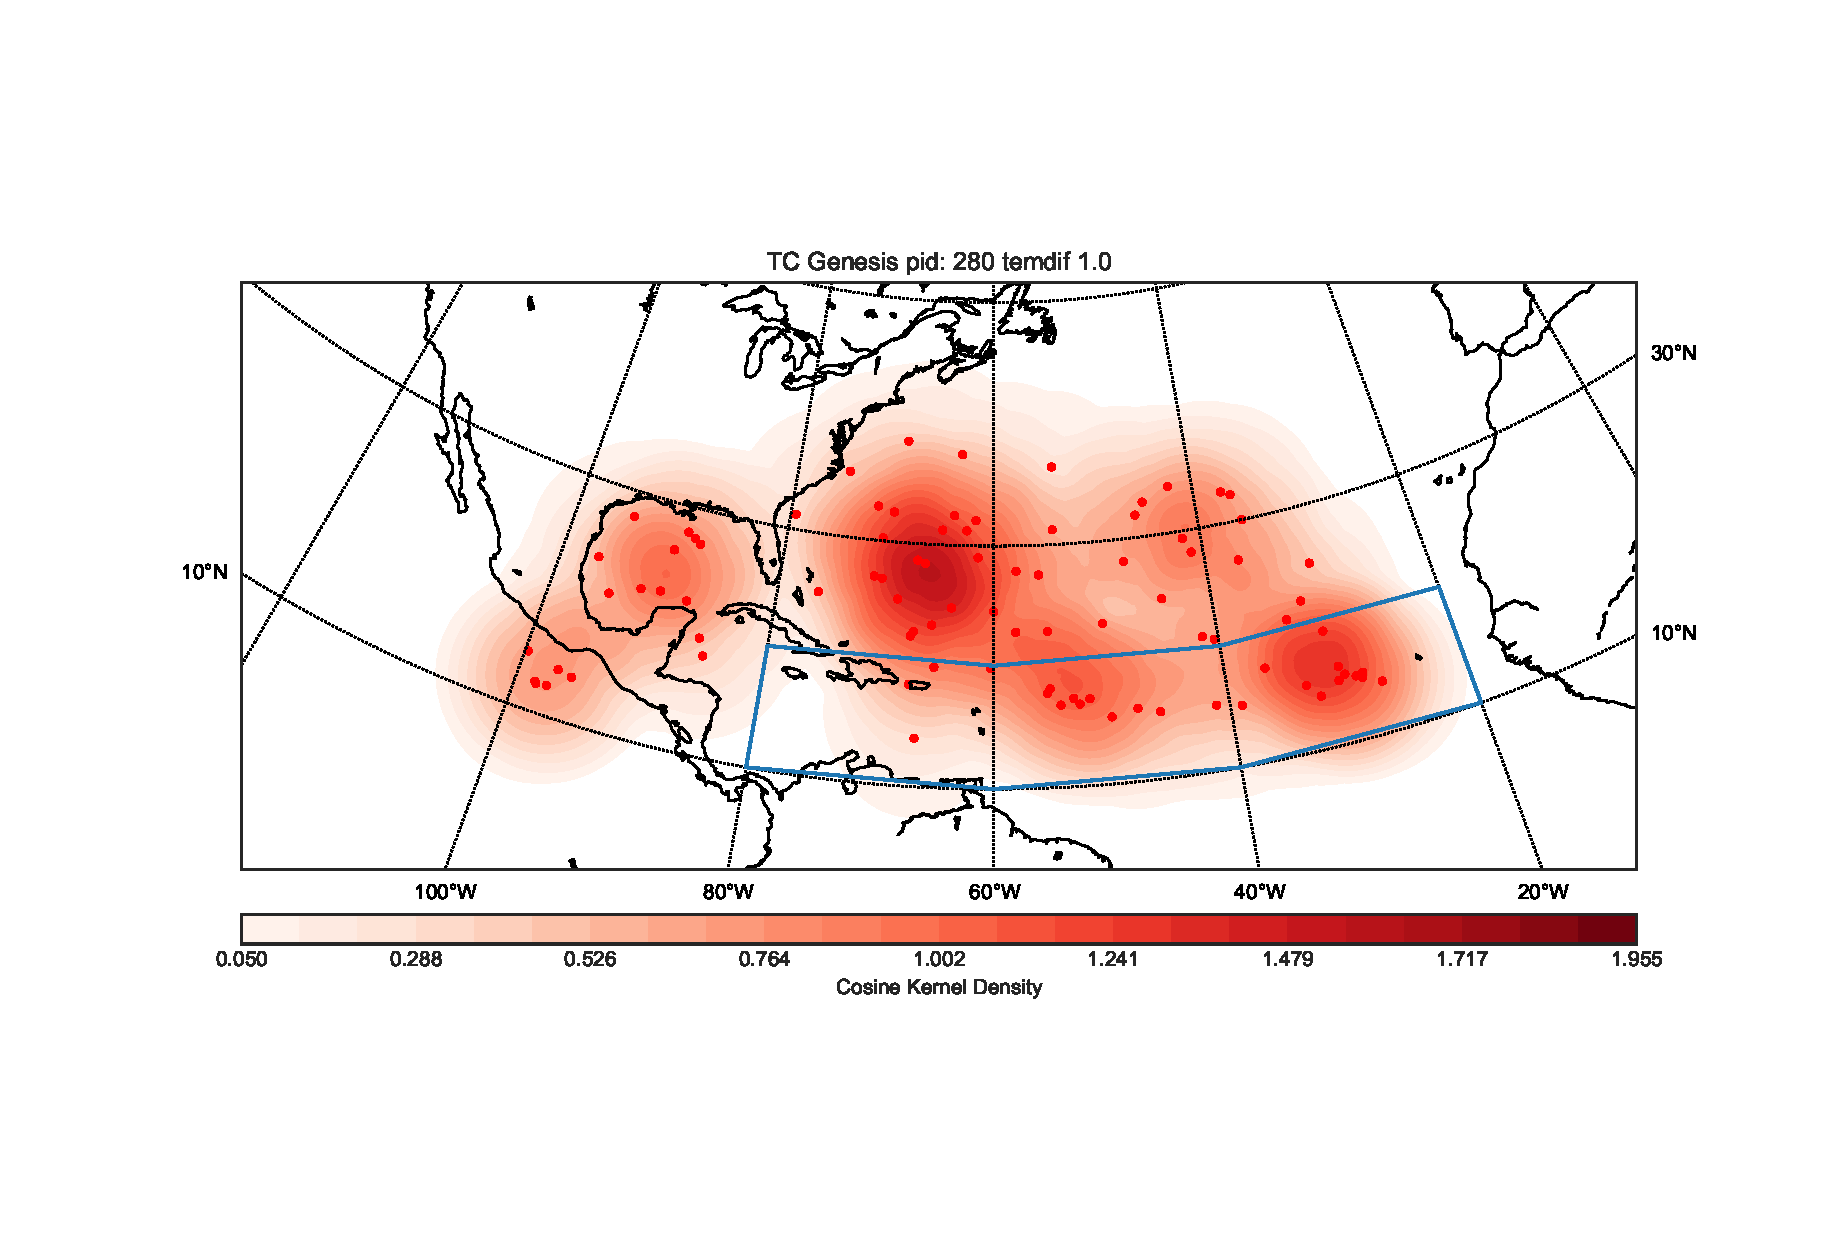
\includegraphics[width=0.7\textwidth]{img/genesis_plot_temdif1.eps}
	\caption{Genesis spots and density for a specific parameter combination.}
	\label{fig:genesis-temdif1}
\end{figure}

\section{Track occurrence frequency }
It has been shown that the choice of parameters affects typical distributions like the lifetime and intensity of the found TCs. With the purpose of assessing the effect of different warm core criteria on the length of the tracks, the point occurrence frequency was visualised. This quantity is the frequency of a specific location at a certain time being recognised as part of a TC track. Specifically, it evaluates to 1 if all parameter combinations determine a point to be a TC and to 0.5 if only the half of them do. The tracks shown in Fig.~\ref{fig:occ-prob} are determined using the parameter combinations from Tab.~\ref{tab:occ-prob-params}.

\begin{table}[ht]
	\centering
	\begin{tabular}{|l|l|l|}
		\hline
		\textbf{parameter} & \textbf{unit} & \textbf{values} \\ \hline
		temdif             & K             & 0.5, 1 ,1.5     \\
		temdis             & m             & 200000          \\
		slpdis             & m             & 100000          \\
		vormin             & 1/s           & $10^{-5}$
		\\
		\hline
	\end{tabular}
	\caption{Parameter combinations used for occurrence frequency plots in Fig.~\ref{fig:occ-prob}.}
	\label{tab:occ-prob-params}
\end{table}
It can be observed that the weaker warm core criterion tracks TCs that are found by only a small part of the parameter combinations. Furthermore, the ends of TC tracks that are found in all of the three plots are longer for the lower values of temdif. Therefore, the weaker warm core criterion enables tracking in earlier development phases. This observation will be made more precise in the following section.
\begin{figure}[ht]
	\centering
	\includegraphics[width=0.6\textwidth]{img/tc_tracks_occ_prob_pid_109_temdif_05.png}
	\\[\smallskipamount]
	\includegraphics[width=0.6\textwidth]{img/tc_tracks_occ_prob_pid_149_temdif_10.png}
	\\[\smallskipamount]
	\includegraphics[width=0.6\textwidth]{img/tc_tracks_occ_prob_pid_189_temdif_15.png}
	\caption{Tracks from all ensemble members for the parameter combinations in Tab.~\ref{tab:occ-prob-params}.}
	\label{fig:occ-prob}
\end{figure}
